% CREATED BY MAGNUS GUSTAVER, 2020
\chapter{Related Work}
\label{chap:related-work}

This chapter positions NanoMem within prior work on LLM agents, long-term
agent memory, retrieval-augmented generation, temporal reasoning, and
reinforcement learning for memory systems. The goal is not to present these
areas as competing lines of work, but to clarify their system boundaries.
NanoMem builds on retrieval and memory-augmented agent research, while focusing
on a narrower problem: constructing compact, source-grounded, temporally
grounded evidence at query time for long-term conversational memory.

\section{LLM Agents}
\label{sec:rw-llm-agents}

Large language model agents extend language models from single-turn text
generators into systems that can act over multiple steps. In this setting, an
LLM is used as a controller that may decompose tasks, call tools, inspect
external observations, update its plan, and produce responses based on both the
current instruction and accumulated state. Work such as ReAct and Toolformer
helped establish the idea that language models can interleave reasoning with
external actions or tool calls rather than only generating a final answer in
one pass \cite{yao2023react,schick2023toolformer}.

Although agent systems vary in implementation, they commonly combine several
functional components: planning, tool use, retrieval, memory, and feedback or
reflection. These components are useful because real tasks often require more
than the information present in the current prompt. An agent may need to
retrieve a document, remember a user preference, revise a plan after an
observation, or decide that more information is needed before answering.

Memory becomes central when the agent is expected to serve the same user,
project, or workflow over a long period of time. A conversational agent cannot
rely only on the current context window if the relevant information was
mentioned days or months earlier. It needs a mechanism for storing and
re-accessing preferences, facts, corrections, plans, events, and task state
across sessions. The remainder of this chapter focuses on that memory problem,
especially in long-term conversational settings.

\section{Long-Term Agent Memory}
\label{sec:rw-long-term-agent-memory}

Long-term agent memory addresses the mismatch between persistent user history
and the limited active context available to an LLM. In a long-running
interaction, useful information is distributed across many sessions and may
include user preferences, personal facts, project decisions, future plans,
outdated statements, corrections, and events mentioned only once. Directly
passing the entire history to the model is expensive, slow, and often
unreliable. A memory system therefore turns past interactions into a resource
that can be stored, maintained, retrieved, and reused when a future query
requires it.

\begin{figure}[H]
  \centering
  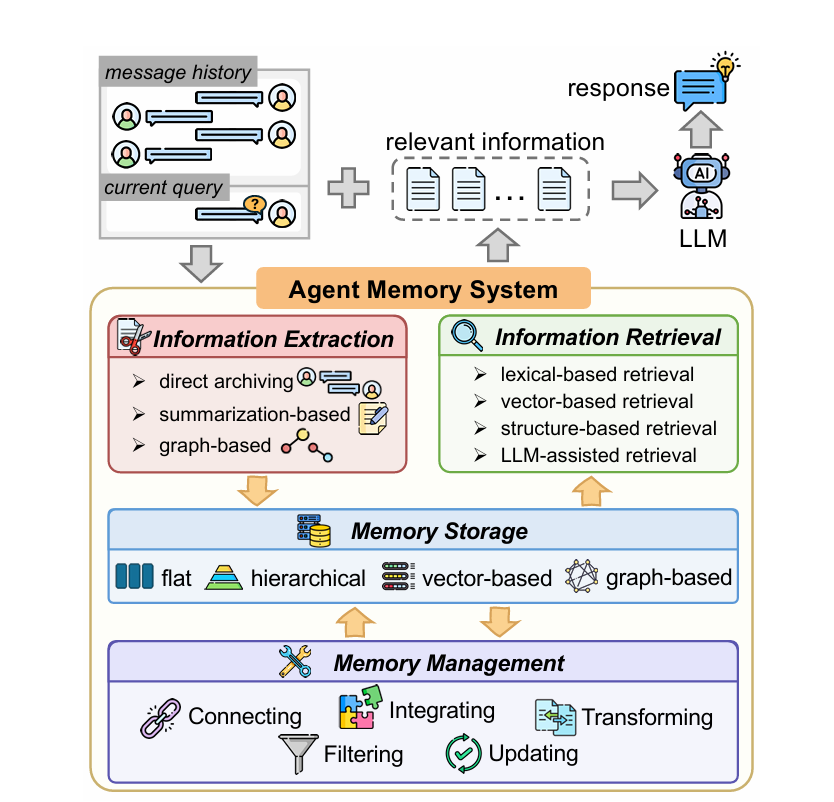
\includegraphics[width=0.88\textwidth]{figure/realted_work_memory_framework.png}
  \caption{A generic long-term agent memory framework. Historical messages and
  the current query are processed by an agent memory system that extracts,
  stores, manages, and retrieves information before passing relevant memory
  content to the LLM.}
  \label{fig:rw-memory-framework}
\end{figure}

Figure~\ref{fig:rw-memory-framework} summarizes a common view of long-term
agent memory. On the write side, information extraction decides how interaction
history enters memory. Some systems directly archive conversations, others
summarize them into compact records, and graph-based systems extract entities,
relations, or events. Memory storage then determines how the resulting memory
units are represented and indexed, for example as flat records, hierarchical
structures, vector stores, or graph stores. Memory management maintains the
memory over time by connecting, integrating, transforming, filtering, and
updating records. On the query side, information retrieval selects relevant
memory content through lexical, vector-based, structure-based, or LLM-assisted
methods.

This framework is useful because it separates two design choices that are often
blurred. A memory system may do heavy write-time processing, attempting to
summarize, normalize, and structure information before a future query is known.
It may also do query-time processing, where the current user question determines
which parts of memory should be retrieved and how they should be interpreted.
NanoMem does not reject write-time processing. It uses lightweight extraction,
temporal enhancement, and indexing so that memories remain searchable. However,
it avoids making the memory writer responsible for heavy interpretation of
future query-dependent relations. The main reasoning step is moved to query
time, where evidence can be constructed with the actual question in view.

Prior long-term memory systems cover several parts of this framework. MemGPT
frames memory as a virtual context management problem, where an agent decides
which information should stay in active context and which should be moved to
external storage \cite{packer2023memgpt}. Production-oriented systems such as
Mem0 and MemOS organize histories into persistent memory units and expose
memory as a reusable service for agents \cite{chhikara2025mem0,li2025memos}.
Structured memory systems enrich the memory substrate itself: Zep uses a
temporal knowledge graph, A-Mem constructs dynamic agentic notes, GMemory
studies hierarchical memory for multi-agent systems, HyperMem uses hypergraph
memory for long conversations, and MemPalace represents a local-first memory
management direction \cite{rasmussen2025zep,xu2025amem,zhang2025gmemory,
yue2026hypermem,mempalace2026}. Compression-oriented systems such as LightMem
and R3MEM reduce the cost of retaining long histories
\cite{fang2025lightmem,wang2025r3mem}.

These systems show that agent memory is not simply a vector database attached
to a chatbot. It is a long-lived subsystem with extraction, storage,
management, and retrieval responsibilities. This thesis focuses on a narrower
case within that space: conversational agent memory. Conversation history has a
session structure, contains updates and corrections, and frequently includes
relative time expressions. The time at which a user mentions an event can
differ from the time at which the event happened. As a result, long-term
conversational memory requires more than storing more history; it requires
query-time interpretation of how past memories relate to the current question.

\section{RAG}
\label{sec:rw-rag}

Retrieval-Augmented Generation (RAG) is the standard paradigm for combining a
language model with external information. Given a query, a retriever selects
relevant documents or passages from an external corpus, and a generator uses
the retrieved context to produce an answer. Classic work such as REALM, DPR,
RAG, FiD, and Atlas established important variants of this retrieve-then-read
pipeline, including learned retrieval, dense passage retrieval, sequence
generation conditioned on retrieved documents, fusion over multiple passages,
and retrieval-augmented few-shot learning \cite{guu2020realm,
karpukhin2020dpr,lewis2020rag,izacard2021fid,izacard2023atlas}.

Recent RAG research has moved beyond one-shot retrieval. Self-RAG trains a
model to decide when to retrieve and critique its own generations, while
SmartRAG jointly learns RAG-related behaviors from environmental feedback
\cite{asai2024selfrag,gao2025smartrag}. Search-R1 and RAG-RL study
reinforcement learning for search and retrieval behavior
\cite{jin2025searchr1,huang2025ragrl}. Other work optimizes retrieval
preferences, faithfulness, and structured search-agent behavior
\cite{yan2025rpo,tang2025ssfo,ji2026treegrpo,zhu2025stratifiedgrpo}. These
directions are important for NanoMem because they show that query-time
retrieval can be adaptive rather than a fixed top-$k$ operation.

However, RAG and long-term conversational agent memory are not the same task.
RAG is usually defined over an external corpus such as documents, webpages,
papers, or search results. The corpus is often treated as already existing, and
the main problem is to retrieve useful context for the current information
need. Conversational agent memory is produced by the interaction between a user
and an agent. It is personal, multi-session, updateable, and part of the agent's
state. The goal is not only to answer a knowledge question, but to preserve
continuity, personalization, and consistency across time.

This distinction becomes sharper for temporal questions. A RAG document may
have metadata timestamps, but standard RAG does not normally separate the time
at which a memory was mentioned from the time at which the event described by
that memory occurred. In long-term dialogue, that separation is often essential.
If a user says in an April 2 session that they travelled to Europe last week,
the session date and the travel date are different. A later question may depend
on the travel week rather than the April 2 mention. Treating the history as an
ordinary document corpus leaves this temporal relation implicit.

NanoMem therefore uses RAG as a technical neighbor, not as the task definition.
It inherits the query-time retrieval idea and is influenced by reflective RAG
and search-agent RL. At the same time, it also has a write-side memory
component: memories are lightly extracted, timestamped, temporally enhanced, and
indexed without aggressively rewriting the original conversational structure.
The central contribution is then placed on the search side. At query time,
NanoMem synthesizes compact, source-grounded evidence with explicit temporal
fields and a binary sufficiency verdict, rather than returning only raw
retrieved passages or a final answer.

\section{Temporal Reasoning in Agent Memory}
\label{sec:rw-temporal-agent-memory}

Temporal reasoning is a core difficulty in long-term agent memory. Dialogue
contains absolute dates, relative expressions, event order, durations, plans,
updates, and implicit dependencies across sessions. Users rarely formulate
queries as exact session lookups. They ask about ``the week after my
promotion'', ``the trip I mentioned last time'', or ``the meeting before I
changed my plan''. Such questions require the system to identify a temporal
anchor, normalize or infer the relevant time window, and often use that window
to retrieve additional evidence.

Benchmarks support this problem framing. TimeBench and Test of Time evaluate
general temporal reasoning abilities and show that LLMs remain brittle when
handling temporal relations and event ordering
\cite{chu2024timebench,fatemi2025testoftime}. LoCoMo evaluates very long-term
conversational memory and includes temporal and multi-hop question types
\cite{maharana2024locomo}. LongMemEval benchmarks chat assistants on
long-term interactive memory, including temporal reasoning, multi-session
reasoning, knowledge updates, and abstention \cite{wu2024longmemeval}. These
benchmarks make temporal reasoning a central capability for memory systems
rather than an optional add-on.

Existing memory systems incorporate time in several ways. Zep encodes temporal
information into a temporal knowledge graph, making time part of the structured
memory substrate \cite{rasmussen2025zep}. TReMu builds time-aware memory with
timeline summaries and combines them with neuro-symbolic reasoning for
multi-session temporal questions \cite{ge2025tremu}. Beyond Dialogue Time
argues for temporal semantic memory that goes beyond the dialogue timestamp
alone \cite{su2026beyonddialoguetime}. Memory-T1 uses reinforcement learning to
improve temporal reasoning in multi-session agents, especially through
temporally relevant session selection and reasoning \cite{du2026memoryt1}.

NanoMem is aligned with these works in treating time as essential, but it uses
time differently. Rather than only storing time as metadata, summarizing it into
a timeline, or using it as a selection signal, NanoMem treats time as part of
the query-time search state. Each synthesized evidence event separates the
source session time from the inferred event time. The inferred event time can
then become a new retrieval cue for the next round. For example, a first round
may find when a user was promoted; the resulting time window can then be used
to search for what the user was reading during that week. This turns temporal
grounding from a passive attribute into an active bridge for multi-hop memory
search.

\section{Reinforcement Learning for Agent Memory}
\label{sec:rw-rl-agent-memory}

Reinforcement learning is relevant to agent memory because many memory
decisions are policy decisions rather than simple next-token prediction
problems. A system may need to learn what to write, what to update, what to
retrieve, whether current evidence is sufficient, whether another search round
is needed, and how compact the intermediate evidence should be. These decisions
are naturally evaluated by downstream usefulness, temporal grounding,
faithfulness, and stop-or-continue behavior.

One line of work applies RL or learnable policies to write-side memory
construction and management. Memory-R1 trains agents to manage and utilize
memories through reinforcement learning, while MemReader and Mem-$\alpha$ study
active or learnable memory construction during the ingestion stage
\cite{yan2025memoryr1,kang2026memreader,wang2025memalpha}. These systems show
that memory operations do not need to be purely hand-written heuristics. Their
focus, however, is primarily on memory construction, extraction, or lifecycle
management before or during storage.

A second line trains search-side behavior for RAG and retrieval agents.
Search-R1, RAG-RL, RPO, SSFO, TreeGRPO, and Stratified GRPO optimize retrieval,
query rewriting, tool use, faithfulness, or multi-step search behavior
\cite{jin2025searchr1,huang2025ragrl,yan2025rpo,tang2025ssfo,ji2026treegrpo,
zhu2025stratifiedgrpo}. MMOA-RAG and EMG-RAG also connect retrieval-augmented
generation with multi-agent RL or editable memory graphs
\cite{chen2025mmoarag,wang2024emgrag}. These works are relevant because they
demonstrate that search behavior can be trained, but their rewards are often
attached to final answer quality, retrieval success, or generic faithfulness
signals rather than to structured memory evidence.

Memory-T1 is closest to NanoMem in that it combines reinforcement learning with
multi-session temporal memory \cite{du2026memoryt1}. The difference is the
trained object and the intermediate output. Memory-T1 primarily improves
temporal session selection and answer behavior. NanoMem trains the Synthesizer
as an evidence construction policy. Its output is not merely an answer or a
selected session, but a set of structured evidence events together with a
binary verdict, \texttt{sufficient} or \texttt{insufficient}. This verdict is
important because hidden-dependency temporal questions often require an
intermediate bridge: the first evidence may be useful because it reveals the
next retrieval cue, even though it is not yet enough to answer the user query.

This framing motivates the method in the next chapter. NanoMem uses
reinforcement learning to optimize intermediate evidence synthesis, with
signals for parseable format, compactness, downstream usefulness, temporal
grounding, and sufficiency behavior. The resulting policy is trained to decide
not only what evidence to state, but also whether the current evidence should
stop the search or guide another retrieval round.
